
\par{
    Ce chapitre présente le cadre institutionnel de notre structure de 
    stage qui est \\LESCAL. Tout d'abord nous présenterons LESCAL (historique, organisation,
    environnement,...) et par la suite le déroulement de notre stage (entités parcourues,
    observation,...)

}

\section{Présentation du LESCAL}
\subsection{ Historique, missions, objectifs et activités du LESCAL}

\subsubsection{Historique du LESCAL}
Le Laboratoire d'Etudes Statistiques et de Conception d'Applications et logiciels,
LESCAL est le fruit de la collaboration entre statisticiens et informaticiens qui
l'ont créé en Juillet 2017. LESCAL autrefois dénommé LES (Laboratoire d'Etudes 
Statistiques) était une initiative dont l'objet était d'apporter un appui aux 
étudiants statisticiens et non statisticiens pour le traitement des données 
(analyses statistiques avancées, différentes régressions, méthodes de prévision) 
dans le cadre de la rédaction de leur mémoire de fin de formation
(licence, master, doctorat).

Deux années plus tard (2019), certains membres de l'équipe, aspirant aux nouvelles
technologies ont étendu les domaines d'intervention du LESCAL au secteur du numérique 
d'où le suffixe « CAL » (Conception d'Applications et Logiciels), ce qui engendra LESCAL.
A nos jours le laboratoire intervient dans les divers domaines que sont : le traitement
et l'analyse des données statistiques, le génie logiciel et l'intelligence artificielle.


\subsubsection{Missions et activités du LESCAL}
LESCAL intervient sur deux principaux volets : le génie logiciel et l'intelligence 
artificielle. Conformément au premier, LESCAL répond aux besoins des entreprises, des 
chercheurs, des professionnels, des particuliers en termes de solutions informatiques 
destinées à divers usages: Business analytics (analyse commerciale), comptabilité, 
facturation, site internet, application mobile, etc.  D'autre part, il conçoit des 
solutions d'intelligence artificielle dans les domaines : reconnaissance visuelle 
(computer vision), compréhension du langage humain (Natural Language Processing).
Par ailleurs à travers son vaste programme LESCAL ACADEMY, il offre aux étudiants,
aux professionnels et au personnel des entreprises une gamme variée de formations 
dans le domaine du numérique et de la science des données et contribue à l'insertion
professionnelle des jeunes par des programmes de stage.


\subsubsection{Objectifs de LESCAL}
LESCAL a pour objectif de:
\begin{itemize}
    \item[$\bullet$] promouvoir la statistique dans tous les secteurs d'activité ; \\	
    \item[$\bullet$] promouvoir les métiers du numérique ;\\
    \item[$\bullet$] aider à la gestion statistique informatisée pour une bonne prise de décision;\\
    \item[$\bullet$] former des cadres compétents et de qualité pour la relève.
\end{itemize} 



\subsection{Organisation, fonctionnement, environnement et localisation \\ géographique du LESCAL}

\subsubsection{Localisation et Organisation}
Situation géographique de la structure\\
Siège : Bénin, Abomey-Calavi\\
Téléphone : (+229) 97 67 57 68\\	
Email: lescal@gmail.com et lescal@lescal-soc.com
\\
 L.E.S.C.A.L. est organisé en Unités de Formation et de Recherche (UFR), ce qui correspond au modèle universitaire, celui-ci se voulant digne des recherches contribuant aux innovations technologiques, voulant accompagner les jeunes étudiants des filières du numérique. Les Unités de Formation et de Recherche dont il est constitué sont les suivantes :
\begin{itemize}
 \item[$\circ$]	UFR Datascience / Intelligence Artificielle
 \item[$\circ$]	UFR Ingénierie logiciels desktops
 \item[$\circ$]	UFR ingénierie applications mobiles
 \item[$\circ$]	UFR ingénierie du web / développement web
\end{itemize}
 Ainsi les étudiants sollicitant un stage ou une formation sont alors insérés dans l'une des Unités de Formation et de Recherche selon leurs talents et leurs aspirations professionnelles.
 Le Laboratoire d'Etudes Statistiques et de Conception d'Applications et Logiciels s'organise pour créer une structure professionnelle et de façon à pouvoir mener à bien les objectifs de l'institution. L'organigramme du laboratoire se présente comme suit :

\begin{figure}[h]
    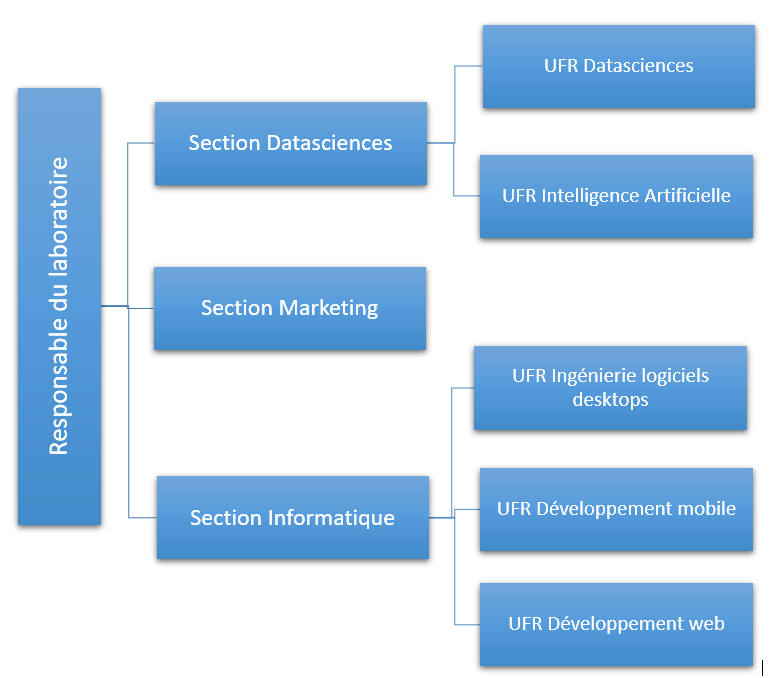
\includegraphics[width=1 \textwidth ]{img/orga.png}
    \caption{Organigramme de LESCAL}
\end{figure}


\subsubsection{Fonctionnement}
LESCAL étant un laboratoire de recherche qui vise à contribuer aux innovations 
technologique, il est subdivisé en quatre grandes Unités de Formation et de 
Recherche (Data sciences / Intelligence Artificielle, ingénierie logiciels 
desktops, ingénierie applications mobiles, ingénierie du web). Le responsable
du laboratoire définit les rôles et attributions de chaque UFR ; chaque UFR
étant dirigée par un sous responsable qui se charge de coordonner les travaux
des membres dans l'atteinte des objectifs généraux du laboratoire.


\subsection{Environnement micro et macro}

\subsubsection{Le micro-environnement}
Le microenvironnement de LESCAL est l'ensemble de tous les éléments qui 
exercent une influence sur les activités du laboratoire, il s'agit de la 
concurrence, la clientèle, les fournisseurs.

\paragraph{La Concurrence}
Le laboratoire L.E.S.C.A.L vit dans un environnement fortement concurrentiel compte tenu de la nature de ses services. Ses concurrents sont l'ensemble des entreprises dont les services sont directement ou indirectement substituables aux siens.
L'analyse de la concurrence étant d'une importance fondamentale pour toute entreprise quelle que soit sa taille, doit lui permettre d'innover, de perfectionner ses produits afin de satisfaire au maximum ses clients et se faire attribuer la plus grande part de marché.

\paragraph{La clientèle}
La clientèle est constiltuée des consommateurs actuels et potentiels qui s'intéressent à 
l'offre du laboratoire. Il s'agit des acheteurs ou consommateurs des services. Elle regroupe 
l'ensemble des opérateurs réels et potentiels des services du laboratoire. En effet, la clientèle 
étant un élément principal de fonds de commerce, toute décision commerciale doit tenir compte de ses 
désirs et attentes.

\paragraph{Les fournisseurs}                                                                  
Il s'agit des entreprises qui fournissent à au laboratoire L.E.S.C.A.L tout ce dont elle
a besoin pour son fonctionnement. Il s'agit des fournisseurs d'intrants, de fournisseurs de 
services généraux (fourniture d'énergies, d'eau, de communications).
Ici, ils représentent les tiers, qui peuvent être des personnes physiques ou morales qui, approvisionnent
la société en prestations diverses.
Ainsi, les fournisseurs peuvent être regroupés en deux (02) catégories :	
\begin{itemize}
    \item[$\circ$] les prestataires de services ;
	\item[$\circ$] les équipementiers.
\end{itemize}		

\subsubsection{Le macro-environnement}
On le définit comme l'ensemble des grandes tendances du laboratoire dans sa globalité. 
La caractéristique et l'évolution du macro-environnement s'imposent au laboratoire: 
en aucun cas, elle n'a la possibilité d'interagir avec. Il s'agit notamment de:


\paragraph{l'environnement politico-légal ou réglementaire} 
Tout comme le marché béninois, l'environnement politico-légal ou réglementaire est aujourd'hui 
fortement marqué par le libéralisme économique.
Au plan législatif, la loi N° 90-005 du 15 mai 1990 fixant les conditions d'exercice des
activités du commerce en République du Bénin affirme les principes de la liberté du 
commerce au Bénin et apporte les allègements substantiels aux procédures d'implantation 
des entreprises commerciales étrangères. 
Au plan réglementaire, les nouveaux textes simplifient les procédures d'exclusion des 
commerçants en rendant plus libre le commerce au Bénin.


\paragraph{L'environnement économique et technologique} 
La définition d'un marché ne tient pas compte seulement de l'aspect quantitatif mais aussi de l'aspect 
qualitatif en terme de pouvoir d'achat des clients actuels et potentiels L'économie béninoise est
actuellement caractérisée par une diminution du pouvoir d'achat de la population due à l'inflation
dont le taux moyen est de 2,5\% en 2005. Selon les données statistiques, une entreprise dont 
l'environnement technologique doit couvrir essentiellement les nouvelles technologies dans les domaines 
de l'information et de la communication et de l'informatique appartenant aux innovations de pointe.


\paragraph{L'environnement démographique et socioculturel} 
Le centre évolue sur un marché à forte croissance à cause de la poussée démographique que connaît le 
Bénin. Avec une superficie de 114 763 $km^2$ et un taux de croissance de 3.25\% selon le Recensement 
Général de la Population et de l'Habitat, la population du Bénin est en plein croissance. Le rythme 
de la croissance démographique présente un intérêt pour le monde des affaires car l'augmentation de 
la population entraîne un accroissement de la demande des offres et donc un développement de ce marché.



